%% ------------------------------------------------------------------------- %%
\chapter{Desenvolvimento Experimental}
\label{cap:desenvolvimentos}

Este trabalho tem o objetivo de explorar possíveis soluções computacionais que sejam capazes de remover ou atenuar a contaminação telúrica de espectros astronômicos capturados a partir do solo. Para fazer isso é necessário um conhecimento aprofundado dos dados coletados, desde os procedimentos adotados na aquisição e redução de dados até interpretações astronômicas de características morfológicas desses sinais.

Neste capítulo são descritos os dados utilizados e os experimentos realizados durante o desenvolvimento do trabalho. Os experimentos foram úteis para permitir a visualização e compreensão dos espectros de ciência e telúrico, o teste do realinhamento de sinais como possível coadjuvante na remoção da contaminação telúrica, e o aprendizado de características fundamentais dos espectros na solução do problema da contaminação telúrica.  


\section{Formato de dados}

% o que é o formato fits
O formato de dados utilizado nos experimentos é o FITS ou \textit{Flexible Image Transfer System}~\citep{pence2010definition}. Este formato de arquivo digital facilita o armazenamento, processamento e transmissão de dados científicos e foi projetado para armazenar conjuntos de dados $n$-dimensionais que consistem em matrizes e tabelas. Este é o formato de dados mais utilizado na astronomia, possuindo recursos específicos para incluir informações de calibração fotométrica e espacial e outros metadados astronômicos relativos aos sinais armazenados.

% composição do arquivo fits
Um arquivo FITS é composto por segmentos chamados de HDU (\textit{Header-Data Units}) e ele deve necessariamente ter um \textit{Primary HDU}, que armazena os dados científicos principais. O \textit{PrimaryHDU} pode ser acompanhado de HDUs adicionais, categorizados entre extensões de imagens, extensões de tabelas ASCII e extensões de tabelas binárias \citep{nasa-fits}.

% header
O \textit{header} de um arquivo FITS contém uma lista de palavras-chave em letra maiúscula, associadas a um valor e possivelmente seguidas de um comentário. Estas palavras-chave representam elementos dos dados que são importantes, como a data de observação do arquivo, seu autor, seu histórico de processamento, seu telescópio de origem e também podem representar elementos relacionados à física da observação, como a massa de ar no momento e local de observação, temperatura ambiente, umidade e etc. A Fig. \ref{fig:fits-header} ilustra o \textit{header} típico de estrelas de ciência. 

\begin{figure}[htb]
\centering
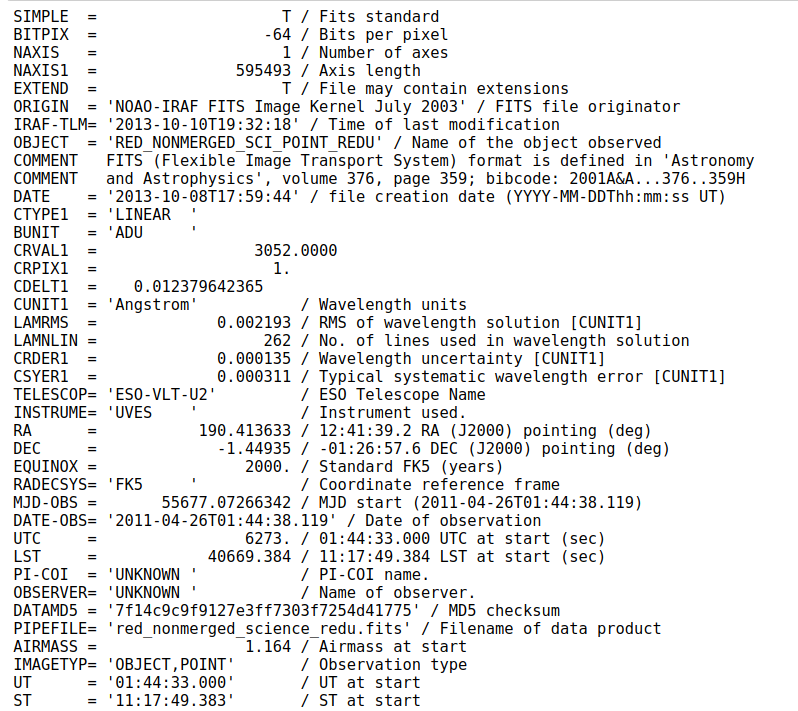
\includegraphics[width=10cm]{figuras/fits_header.png}
\caption{Trecho do cabeçalho do arquivo FITS da estrela HD110379}
\label{fig:fits-header}
\end{figure}

% data e tipos de dados
Dentro de uma HDU em um arquivo FITS, o componente em sequência ao \textit{header}, quando presente, possui um vetor que pode ter desde 1 até 999 dimensões. Esta seção representa o dado astronômico capturado, como os valores do fluxo de um espectro estelar ou uma imagem de um objeto celeste. Os dados podem ter um de 5 possíveis tipos de dados \citep{pence2010definition}:

\begin{enumerate}
    \item Inteiros de 8 bits
    \item Inteiros de 16 bits
    \item Inteiros de 32 bits
    \item Números reais de ponto flutuante de 32 bits
    \item Números reais de ponto flutuante de 64 bits
\end{enumerate}

\section{Ambiente e ferramentas}

%introduzir seção
A realização dos experimentos deste trabalho foi dependente de um conjunto de bibliotecas especializadas. Esta seção descreve as ferramentas utilizadas e detalhes da implementação dos experimentos.

% linguagem de programação: python
A linguagem de programação de escolha para a implementação dos experimentos foi o \textit{Python}, por esta permitir o uso de bibliotecas especializadas para o processamento de sinais e manipulação de dados astronômicos.

% jupyter notebooks
Os experimentos foram implementados em \textit{notebooks} do \textit{Jupyter}\footnote{\url{https://jupyter.org/}} \citep{Kluyver:2016aa}, um projeto de código-aberto com o objetivo de oferecer suporte à ciência de dados e computação científica interativa. Neste ambiente computacional é possível escrever código em células que podem ser executadas de forma independente. Esta interatividade faz com que os \textit{notebooks} sejam ambientes perfeitos para uma programação de natureza exploratória, já que é possível executar experimentos e apresentar resultados e gráficos entre várias células de código.

% pacotes python
Estabelecidos a linguagem e o ambiente dos experimentos, foram usadas diversas bibliotecas de \textit{Python} para ler, manipular e visualizar os dados estelares. Os pacotes utilizados foram: o \textit{NumPy}\footnote{\url{https://numpy.org/}} \citep{oliphant2006guide}, uma biblioteca fundamental de computação científica performática com suporte para vetores e matrizes grandes e multidimensionais, além de diversas funções matemáticas de alto nível; o \textit{Matplotlib}\footnote{\url{https://matplotlib.org/}} \citep{Hunter:2007}, uma biblioteca gráfica que permite a visualização de dados em diversos tipos de gráficos; e finalmente o \textit{Astropy}\footnote{\url{http://www.astropy.org}} \citep{astropy:2018}, uma biblioteca que é amplamente usado para processar computacionalmente diversos dados astronômicos e tem funcionalidades como leitura de arquivos FITS, conversões de unidades e quantidades físicas e computações cosmológicas.

\section{Conjuntos de dados}

% datasets fornecidos: ardata, uves, molecfit e xsl (principal conjunto de dados)
Para o desenvolvimento dos experimentos destre trabalho, foram obtidos alguns conjuntos de dados estelares. Todos os arquivos destes conjuntos estão no formato FITS. Estes conjuntos de dados estelares englobam tanto observações reais de estrelas quando espectros telúricos sintéticos. A lista a seguir descreve estes conjuntos.

% lista dos dados 
\begin{itemize}
    \item UVES: dois pares de arquivos FITS contendo observações das estrelas HD110379 e HD110379 e seus respectivos referenciais telúricos. Estes dados foram capturados pelo espectrógrafo UVES \footnote{\url{https://www.eso.org/sci/facilities/paranal/instruments/uves.html}} \citep{2000SPIE.4008..534D}, parte do \textit{Very Large Telescope Array} \footnote{\url{https://www.eso.org/public/brazil/teles-instr/paranal-observatory/vlt/?lang}}, no Cerro Paranal, Chile.
    \item FTS: uma tabela FITS contendo observações reais do Sol, da estrela Arcturus e um referencial telúrico para ambas.
    \item XSL: dados de observações do \textit{X-Shooter} \citep{Chen2014TheXS}, outro espectrógrafo que compõe o \textit{Very Large Telescope Array}. Mais detalhes sobre este conjunto de dados são explicados nesta seção (Anaïs Gonneau, comunicação privada).
    \item Molecfit: dados telúricos sintéticos gerados com a ferramenta Molecfit \citep{smette2015molecfit} 
\end{itemize}

% leitura dos dados
Antes de qualquer teste foi necessário um processo de ambientação e familiarização com os dados astronômicos. Para a leitura e manipulação de dados no formato FITS foi usada a biblioteca \textit{Astropy}.

% exemplos de estrelas mencionadas acima
A combinação dos dados com o ferramental adequado, possibilitou analisar e visualizar o espectro de diversas estrelas. Dois exemplos de estrelas de ciência e seus referenciais telúricos estão nas figuras~\ref{fig:two-stars-hd110379} e~\ref{fig:two-stars-sun}, e representam, respectivamente, a estrela HD110379 e o Sol. Além dos espectros completos, a figura~\ref{fig:two-stars-zoom-hd110379} ilustra dois painéis aumentados dos espectros observado e telúrico de HD110379, asim é possível ver as linhas espectrais com mais detalhes e compreender qual informação é perdida para a contaminação telúrica.

% observado e o telurico de cada um (ardata e uves)
\begin{figure}[!htb]
  \centering
  \subfloat[HD110379]{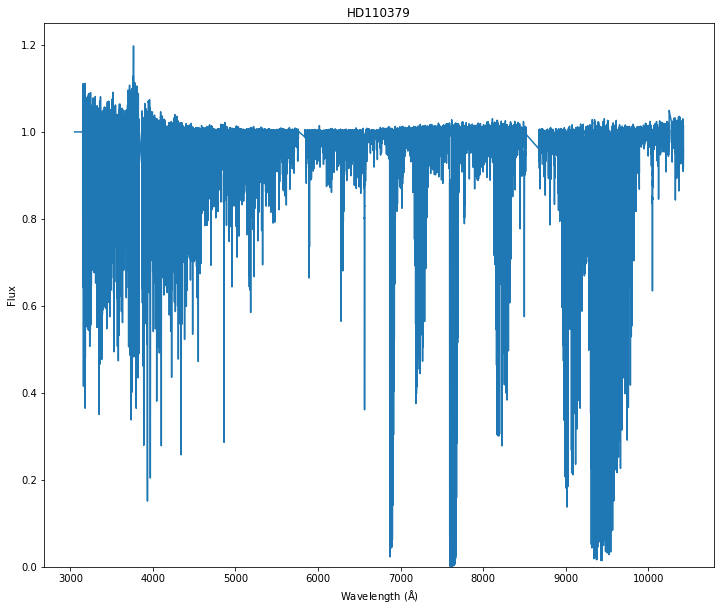
\includegraphics[width=0.5\textwidth]{figuras/hd110379_spectrum.png}\label{fig:hd110379}}
  \hfill
  \subfloat[Referência telúrica para HD110379]{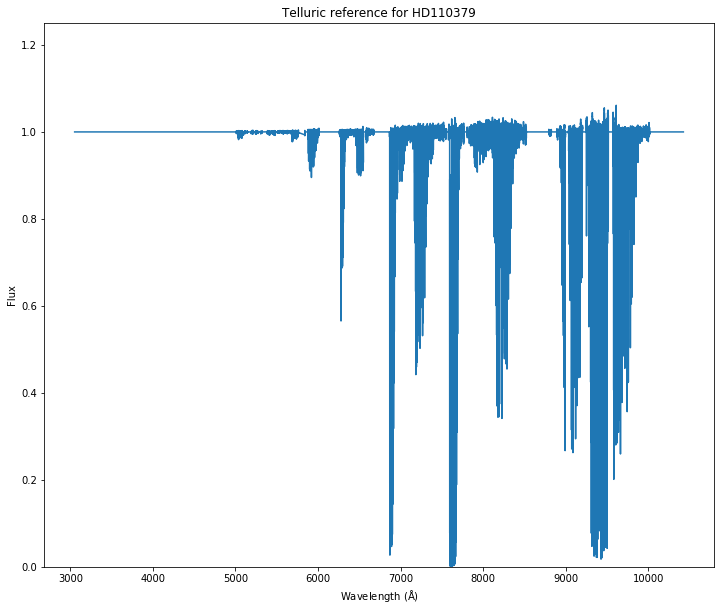
\includegraphics[width=0.5\textwidth]{figuras/hd110379_telluric.png}\label{fig:hd110379-tel}}
  \caption{Espectro observado com contaminação e espectro telúrico de HD110379}
  \label{fig:two-stars-hd110379}
\end{figure}

\begin{figure}[!htb]
  \centering
  \subfloat[HD110379]{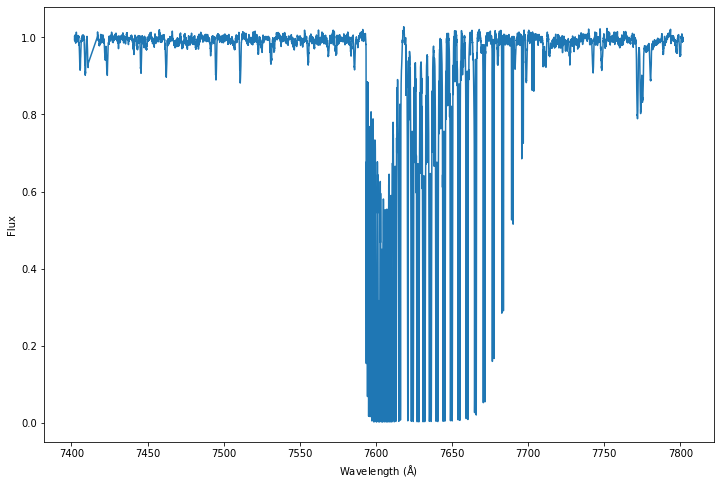
\includegraphics[width=0.5\textwidth]{figuras/hd110379_spectrum_zoom.png}\label{fig:hd110379-zoom}}
  \hfill
  \subfloat[Referência telúrica para HD110379]{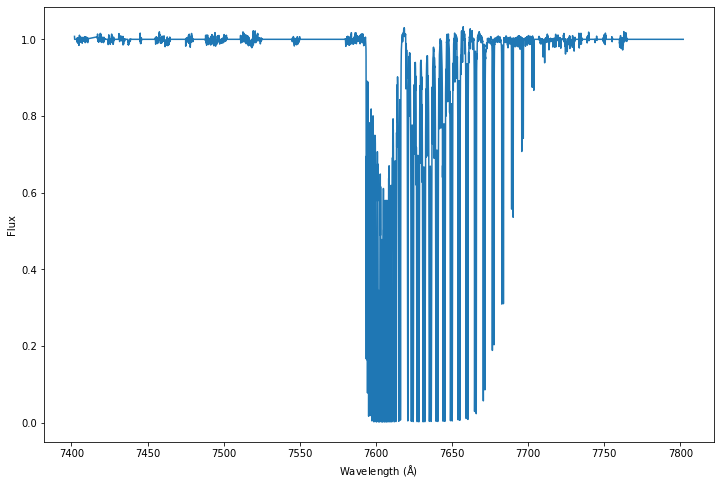
\includegraphics[width=0.5\textwidth]{figuras/hd110379_telluric_zoom.png}\label{fig:hd110379-tel-zoom}}
  \caption{Parte do espectro observado com contaminação e espectro telúrico de HD110379 no intervalo de comprimento de onda de 7400\mathrm{\AA} a 7800\mathrm{\AA}}
  \label{fig:two-stars-zoom-hd110379}
\end{figure}

\begin{figure}[htb]
  \centering
  \subfloat[Sol]{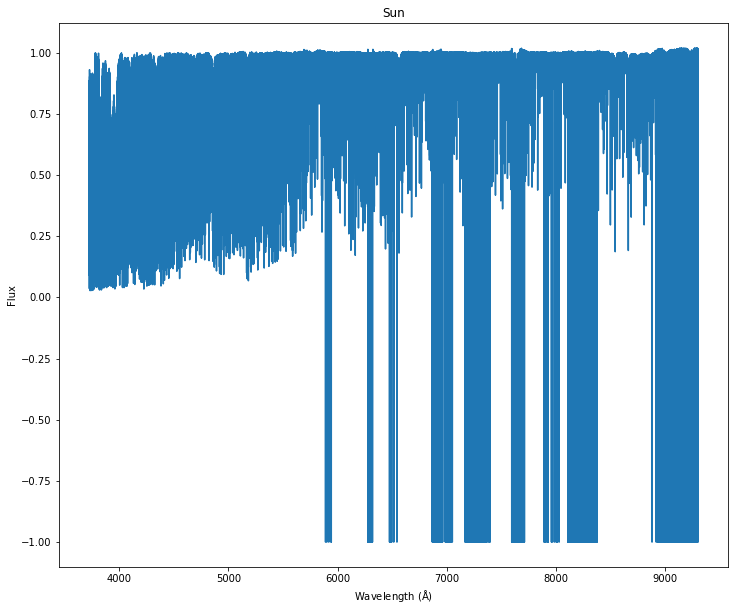
\includegraphics[width=0.5\textwidth]{figuras/sun_spectrum.png}\label{fig:sun}}
  \hfill
  \subfloat[Referência telúrica para o Sol]{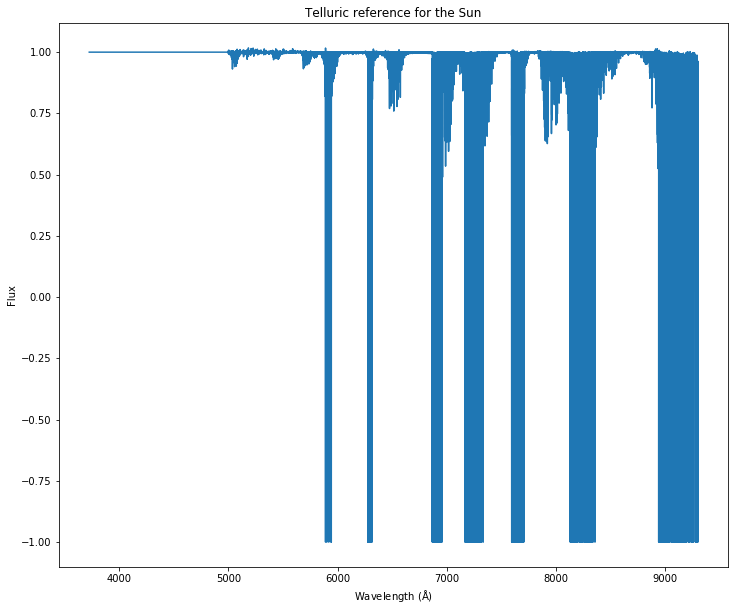
\includegraphics[width=0.5\textwidth]{figuras/sun_telluric.png}\label{fig:sun-tel}}
  \caption{Espectro observado com contaminação e espectro telúrico do Sol}
  \label{fig:two-stars-sun}
\end{figure}

% \mqz{Na figura 3.3 do Sol, o item (a) não é um espectro contaminado? O termo ``estrela de ciência'' é adequado para se referir a esse espectro?}

% seleção do xsl como dataset principal
Além das estrelas acima, como foi mencionado na seção~\ref{similarity-and-signal-alignment}, o principal conjunto de dados utilizado nos experimentos deste trabalho são estrelas do \textit{X-Shooter Spectral Library}. O diferencial deste conjunto de dados é que além das observações estelares e referenciais telúricos, foram fornecidos os espectros resultantes da correção telúrica. Desta maneira, foi possível estabelecer um \textit{ground truth} como base de comparação para os resultados dos experimentos. Neste conjunto de dados foram fornecidas quatro estrelas (X0319, X0386, X0538, X0771), com nove arquivos cada, distribuídos da seguinte maneira:

% mais detalhes sobre os dados do xsl (4 estrelas de ciencia, 4 teluricas sinteticas do molecfit e 4 corrigidas, dividas entre as regioes do espectro eletromagnetico infravermelho, visivel, ultravioleta)
\begin{itemize}
    \item *X\_N\_E.fits ou *X\_O\_E.fits: o espectro da estrela com contaminação telúrica, separado em 3 arquivos que cobrem intervalos de comprimento de ondas diferentes (X no nome do arquivo será U = ultravioleta, V = visível ou N = infravermelho);
    \item *TRA.fits: modelo Molecfit que representa o espectro telúrico correspondente ao dia da observação, também separado em 3 arquivos que cobrem comprimentos de ondas diferentes;
    \item *TAC.fits ou *TAC\_final.fits: espectros das estrelas corrigidos pelo modelo Molecfit e já considerando que as distorções observadas em comprimento de onda foram corrigidas, também separado em três arquivos.
\end{itemize}

% desnecessário:
%\noindent o que resulta em 36 arquivos no total.

% plotar os espectros do xsl nas unidades que vieram e falar das diferenças entre os obs e teluricos (escalase formatos) e diferenca com figuras anteriores
\begin{figure}[htb]
  \centering
  \subfloat[X0319 observado]{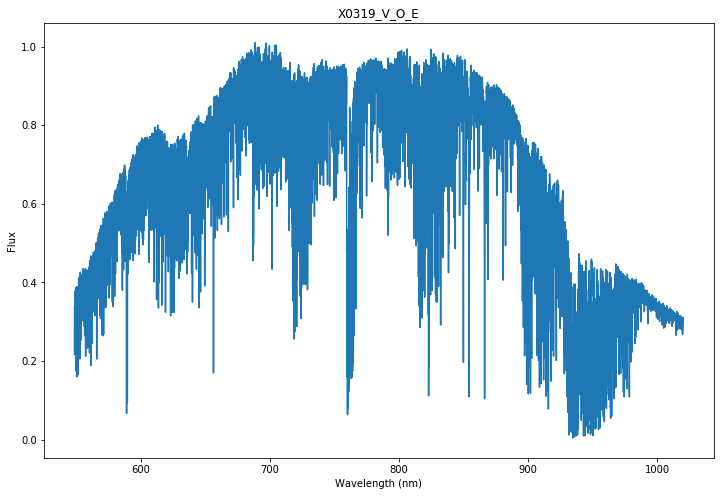
\includegraphics[width=0.5\textwidth]{figuras/x0319_v_o_e.png}\label{fig:x0319-v-o-e}}
  \hfill
  \subfloat[Referência telúrica para X0319]{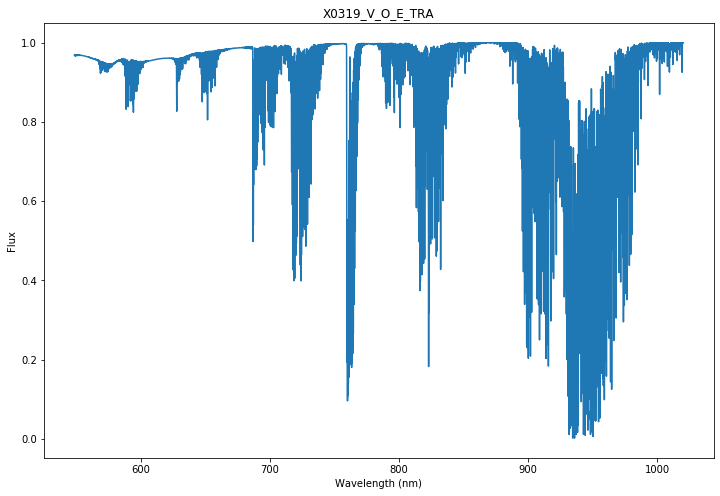
\includegraphics[width=0.5\textwidth]{figuras/x0319_v_o_e_tra.png}\label{fig:x0319-v-o-e-tra}}
  \caption{Espectro observado com contaminação e espectro telúrico de X0319 na região visível de comprimento de onda}
  \label{fig:x0319-visible}
\end{figure}


\begin{figure}[htb]
  \centering
  \subfloat[X0386 observado]{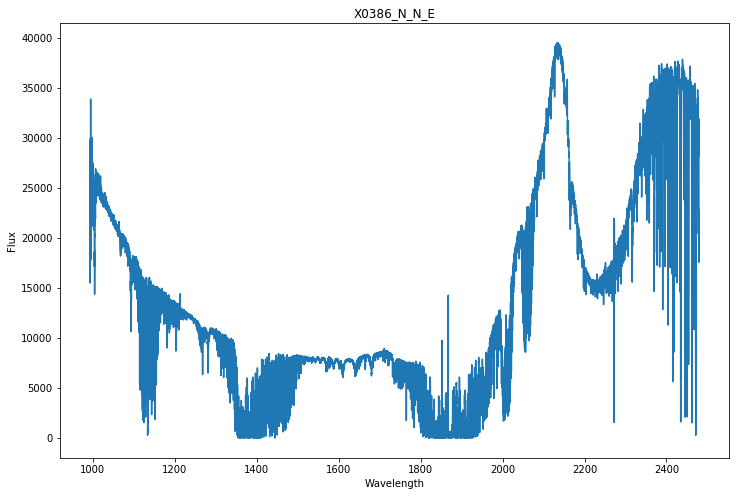
\includegraphics[width=0.5\textwidth]{figuras/x0386_n_n_e.png}\label{fig:x0386-n-n-e}}
  \hfill
  \subfloat[Referência telúrica para X0386]{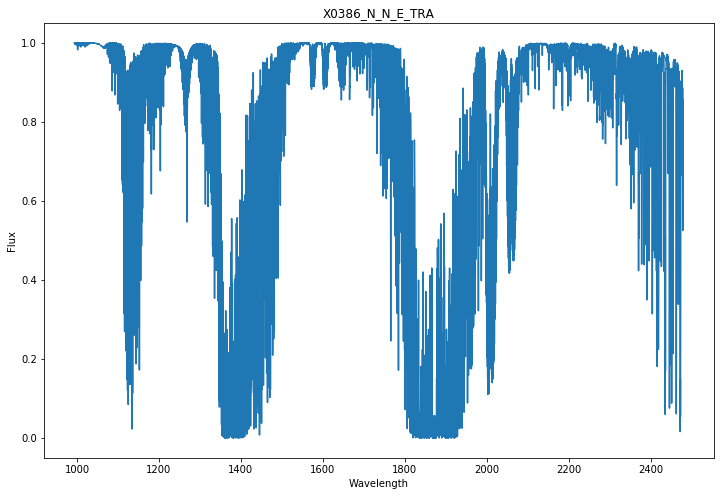
\includegraphics[width=0.5\textwidth]{figuras/x0386_n_n_e_tra.png}\label{fig:x0386-n-n-e-tra}}
  \caption{Espectro observado com contaminação e espectro telúrico de X0386 na região infravermelho de comprimento de onda}
  \label{fig:x0386-infrared}
\end{figure}


\begin{figure}[htb]
  \centering
  \subfloat[X0538 observado]{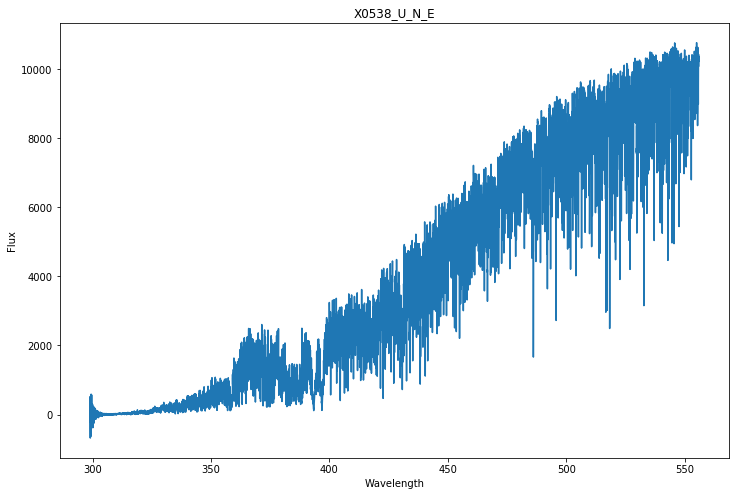
\includegraphics[width=0.5\textwidth]{figuras/x0538_u_n_e.png}\label{fig:x0538-u-n-e}}
  \hfill
  \subfloat[Referência telúrica para X0538]{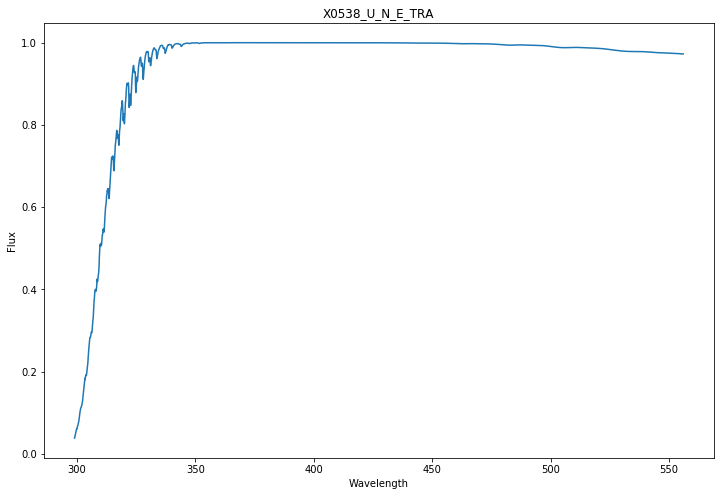
\includegraphics[width=0.5\textwidth]{figuras/x0538_u_n_e_tra.png}\label{fig:x0538-u-n-e-tra}}
  \caption{Espectro observado com contaminação e espectro telúrico de X0538 na região ultravioleta de comprimento de onda}
  \label{fig:x0538-ultraviolet}
\end{figure}

As figuras~\ref{fig:x0319-visible},~\ref{fig:x0386-infrared} e~\ref{fig:x0538-ultraviolet} ilustram exemplos de alguns espectros do conjunto de dados do \textit{X-Shooter}, tanto de diferentes estrelas quanto de diferentes regiões de comprimentos de onda. 

% falar sobre diferença no eixo y 
Uma das diferenças entre o espectro observado e o telúrico de uma mesma estrela é a diferença de ordem de magnitude da escala do eixo y dos gráficos. Como foi mencionado na seção~\ref{data-reduction}, os espectros observados possuem uma unidade física ao final do processo de redução de dados. No caso das observações do conjunto de dados do \textit{X-Shooter}, os espectros não passaram pelo processo de redução de dados por completo, o que significa que o eixo y não possui o mesmo significado físico de intensidade por unidade de área, tempo e comprimento de onda. 

% tentar introduzir o significado do eixo e explicação da adimensionalidade do fluxo antes do final da redução de dados
Como o fluxo é capturado pelo CCD através da corrente elétrica produzida por uma certa contagem de fótons, o processo de conversão entre a tensão produzida no instrumento e finalmente uma unidade fisicamente interpretável é extremamente sofisticado em termos de \textit{hardware} e não será abordado neste trabalho. Para os experimentos realizados neste capítulo é importante notar que o eixo y é relacionado tanto ao fluxo da estrela quanto à assinatura instrumental do espectrógrafo. 

% espectro do molecfit e normalização pro intervalo [0,1]
Já nos espectros telúricos sintéticos do Molecfit, o eixo y do gráfico é normalizado para o intervalo $[0, 1]$ e representa um mapa de transmitância da atmosfera, ou seja, uma série de fatores de absorção que quando interagem com o sinal estelar capturam parte da sua emissão. Para facilitar o restante dos experimentos, as observações do \textit{X-Shooter} também tiveram seus intervalos normalizados de forma a simplificar a manipulação dos dados.

\section{Divisão do sinal estelar pelo telúrico}

% introdução à motivação por tras deste experimento
% queremos validar com os dados em maos que a divisão de fato não é a melhor solução para o problema e entender qual seria a consequencia dela nestas observações
Após o processo de exploração e familiarização com os dados astronômicos fornecidos, o primeiro experimento idealizado neste trabalho foi a divisão dos espectros estelares observados pelas suas respectivas referências telúricas, a fim de evidenciar as limitações desse processo.
% recapitular pq podemos dividir os espectros
Como mencionado na seção~\ref{telluric-contamination}, por causa da natureza multiplicativa do modelo físico da transmissão da radiação estelar através da atmosfera, a correção telúrica corresponderia de fato à divisão simples entre os espectros de ciência e telúrico. A motivação por trás deste experimento é observar que na prática esta solução não é ideal e cria artefatos no espectro estelar. 

Algumas explicações do porquê o método da correção telúrica pela divisão simples de espectros não funciona como proposto no modelo teórico provêm das distorções do sinal que possuem origem instrumental. Alguns exemplos de distorções esperadas pelos astrônomos em suas observações são o alargamento das linhas espectrais, desconsiderando o alargamento Doppler \citep{LEVENHAGEN2008}, e a criação de deslocamentos no domínio de comprimento de onda.
% mostrar resultados de alguns conjuntos de dados que ilustrem bem a criação de artefatos 
A primeira divisão realizada foi do conjunto de dados do espectrógrafo UVES, na estrela HD110379. 

\begin{figure}[htb]
  \centering
  \subfloat[HD110379]{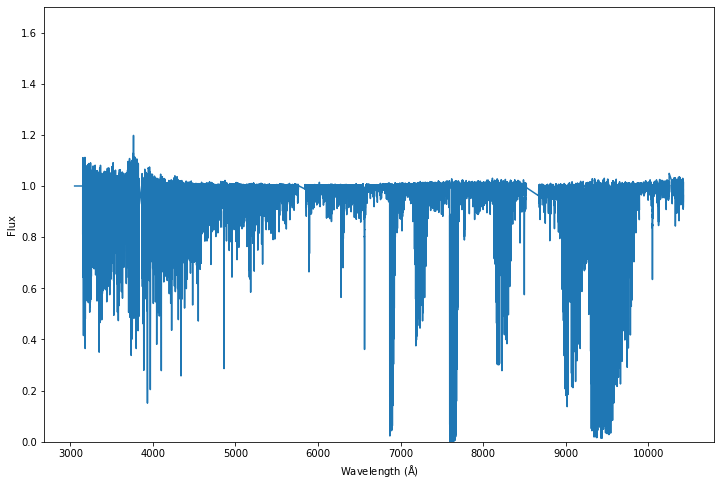
\includegraphics[width=0.5\textwidth]{figuras/hd110379_spectrum_scaled.png}\label{fig:hd110379-spectrum-scaled}}
  \hfill
  \subfloat[Resultado da correção telúrica HD110379]{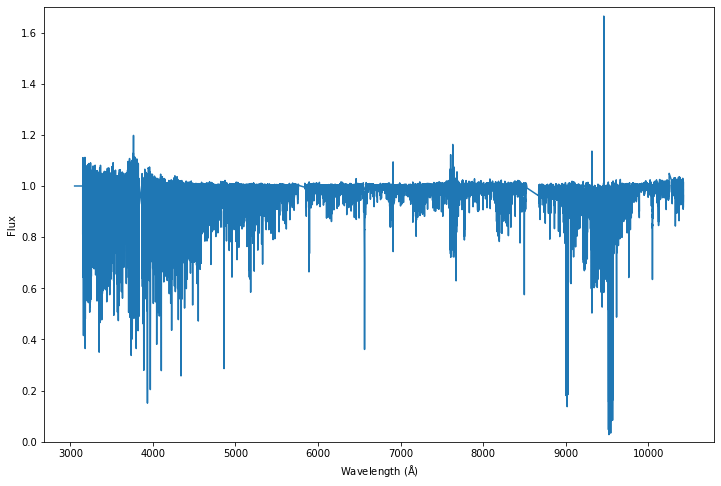
\includegraphics[width=0.5\textwidth]{figuras/hd110379_divided.png}\label{fig:hd110379-divided}}
  \caption{Espectros de ciência e dividido de HD110379 pelo seu referencial telúrico}
  \label{fig:hd110379-division}
\end{figure}

Na figura~\ref{fig:hd110379-division}, temos o espectro de ciência original da estrela HD110379 e o resultado da correção telúrica que é a divisão simples entre os espectros. Ambos tiveram seus eixos y redimensionados de modo a facilitar a inspeção visual dos resultados.  A correção telúrica neste caso de fato diminui algumas das linhas de absorção do espectro, principalmente na região dos 6500$\mathrm{\AA}$ aos 8500$\mathrm{\AA}$ de comprimento de onda. Porém, é visivelmente perceptível que ela também cria artefatos como picos no espectro resultante, sendo alguns menores e outros maiores quando comparados ao intervalo [0, 1] do fluxo estelar.

\begin{figure}[htb]
  \centering
  \subfloat[X0319]{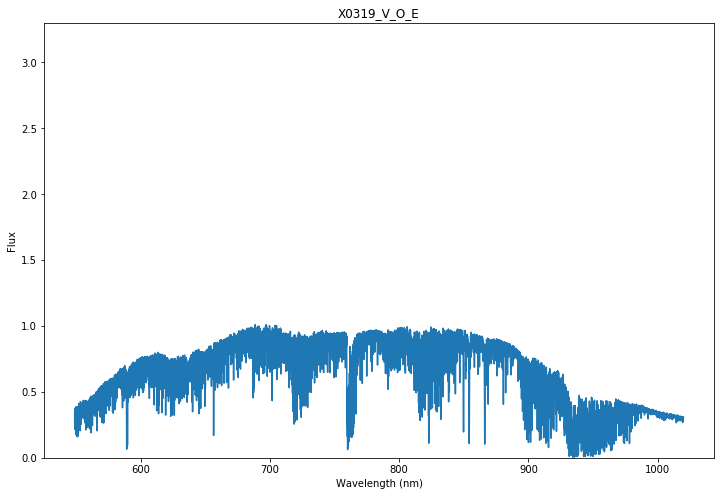
\includegraphics[width=0.5\textwidth]{figuras/x0319_v_o_e_scaled.png}\label{fig:x0319-spectrum-scaled}}
  \hfill
  \subfloat[Resultado da correção telúrica X0319]{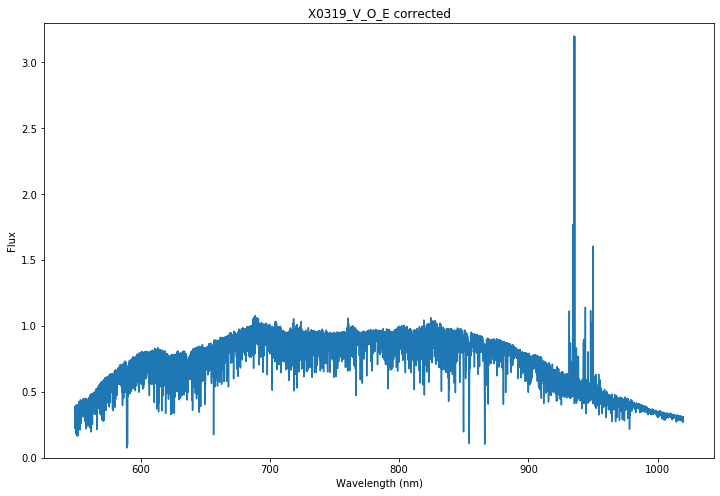
\includegraphics[width=0.5\textwidth]{figuras/x0319_v_o_e_divided.png}\label{fig:x0319-divided}}
  \caption{Espectros de ciência e dividido de X0319 pelo seu referencial telúrico}
  \label{fig:x0319-division}
\end{figure}

A figura~\ref{fig:x0319-division} mostra mais um exemplo de correção telúrica feita nos dados fornecidos, desta vez na estrela X0319 do espectrógrafo \textit{X-Shooter}. Novamente, os eixos dos gráficos dos espectros foram redimensionados, de modo a facilitar a visualização dos efeitos da divisão do observado pelo telúrico. Neste caso, é possível observar tanto a diminuição das linhas de absorção ao longo do espectro, quanto a criação de picos no mesmo, principalmente na região entre 900nm e 1000nm, na qual o pico resultante tem uma escala aproximadamente três vezes maior que a do espectro original.

% picos de sinal podem ter sido causados pos shifts em regiões do espectro
Os artefatos criados pelas correções telúricas das figuras acima não deveriam existir na situação ideal do problema, onde, elemento a elemento, o fluxo do espectro de ciência deveria ser maior ou igual ao fluxo após a absorção atmosférica representada pelo espectro telúrico. Isto indica a presença de um dos efeitos esperados deste tipo de operação: o desalinhamento entre o espectro estelar e o telúrico. Os resultados das correções telúricas e os seus efeitos resultantes fazem sentido, principalmente no caso da estrela do \textit{X-Shooter}, onde pesquisadores observaram estes mesmos problemas \citep{unpublished-xshooter-data-release, wavelength-shifts}

% passar pra dtw e a tentativa de resolver os desalinhamentos
Os resultados das divisões nesta seção ilustram as dificuldades conhecidas no processo atual de correção telúrica e deixam explícita a necessidade propor soluções alternativas que melhorariam a qualidade dos dados observados.

\section{DTW no sinal estelar}

% introdução da seção
Os resultados do experimento de correção telúrica através da divisão de um espectro estelar pelo seu referencial telúrico esclarecem a necessidade de pensar em melhorias ao processo atual. Como foi visto, um dos problemas nos dados é a falta de alinhamento entre os sinais, e a consequente criação de artefatos e distorções nos espectros corrigidos. O experimento desta seção propõe uma solução alternativa a uma das dificuldades conhecidas das observações: o desalinhamento dos espectros.

% MQZ parou aqui.

% decisão de usar dtw
Como foi explicado na seção~\ref{similarity-and-signal-alignment}, podemos usar o algoritmo \textit{Dynamic Time Warping} para encontrar o alinhamento ótimo entre dois sinais. Assim, seria possível realinhar o espectro da observação estelar com o espectro telúrico para resultar em uma divisão de maior qualidade e menor perda de informação e criação de artefatos. 

% dados utilizados no experimento e versão da dtw
Para este experimento o conjunto de dados utilizado foi o XSL e a implementação do DTW foi a \textit{FastDTW}, de modo a conseguir aplicar o algoritmo nos espectros inteiros e maximizar sua performance.

% primeiro experimento
O primeiro exemplo da aplicação da DTW nos dados da XSL é no intervalo visível de comprimento de onda da estrela X0319, cujos espectros são ilustrados na figura~\ref{fig:x0319-visible}. O algoritmo foi aplicado nos espectros estelar e telúrico inteiros, e o caminho gerado pela DTW algoritmo está na figura~\ref{fig:x0319-warp-path}.

\begin{figure}[htb]
\centering
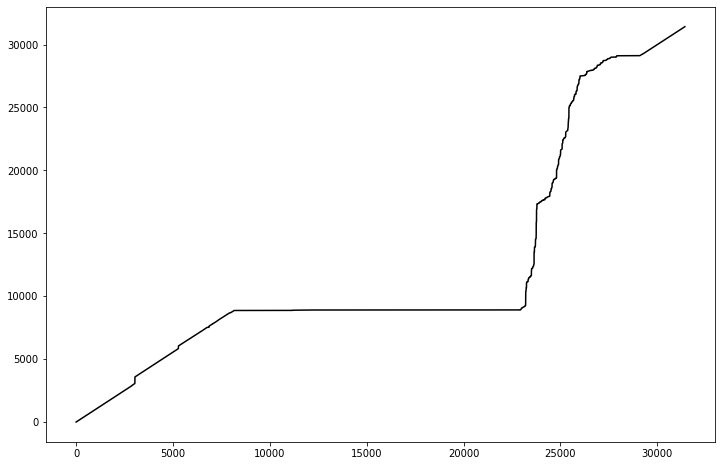
\includegraphics[width=10cm]{figuras/x0319_warp_path.png}
\caption{Caminho da DTW para o espectro estelar e telúrico de X0319}
\label{fig:x0319-warp-path}
\end{figure}

O caminho resultante do algoritmo já indica uma série de regiões problemáticas dos espectros que não puderam ser alinhadas de maneira ótima. Idealmente o caminho deveria se distanciar pouco da diagonal secundária da matriz de similaridade, mas neste caso são claras as regiões onde as sequências não são similares, como a linha horizontal que ocupa a maioria do caminho, seguida de um avanço quase vertical.

O espectro telúrico original do Molecfit e o realinhado em relação à observação estelar que foi reconstruído a partir do caminho da DTW estão na figura~ \ref{fig:x0319-realigned-telluric}.

\begin{figure}[htb]
  \centering
  \subfloat[Modelo telúrico do Molefit de X0319]{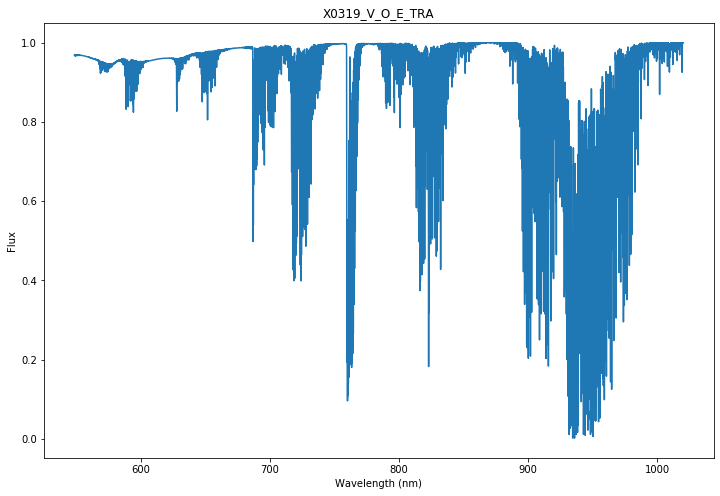
\includegraphics[width=0.5\textwidth]{figuras/x0319_v_o_e_tra.png}}
  \hfill
  \subfloat[Espectro telúrico de X0319 realinhado]{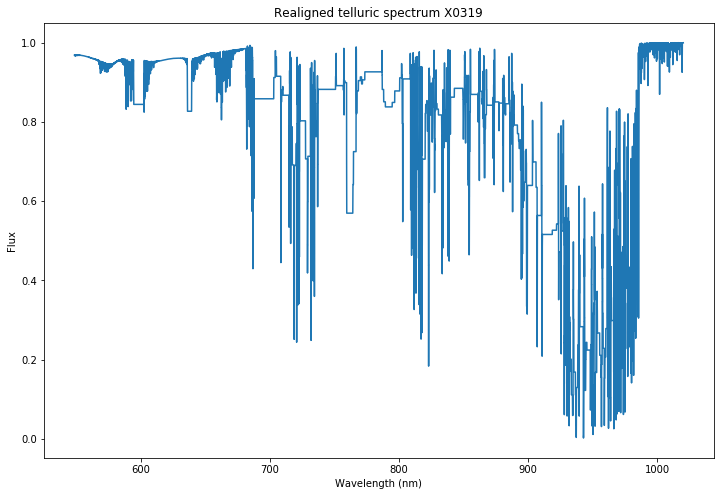
\includegraphics[width=0.5\textwidth]{figuras/x0319_v_o_e_aligned.png}}
  \caption{Espectro telúrico de X0319 e espectro telúrico realinhado a partir do caminho da DTW}
  \label{fig:x0319-realigned-telluric}
\end{figure}

% resultado do espectro telurico realinhado
É possível ver que o espectro telúrico realinhado da estrela X0319 tem um formato muito diferente do modelo do Molecfit. O espectro resultante tem uma forte distorção em relação ao seu formato original e exibe a formação de ângulos retos nas linhas espectrais.

% mais um exemplo em outra estrela no espectro completo

% mais um exemplo com zoom no espectro para mostrar as linhas e os efeitos no nível micro (falar que a contaminação é subpixel)
Uma hipótese do motivo pelo qual a aplicação do DTW no espectro como um todo não mostrou bons resultados é que os desalinhamentos em diferentes regiões não são os mesmos pixel a pixel. Assim, mostrou-se necessário testar o algoritmo de realinhamento em regiões menores do espectro. Foi aplicado o DTW no espectro da estrela X0319, no intervalo de comprimento de onda entre 834nm e 841nm e as figuras~\ref{fig:x0319-warp-path-zoom} e~\ref{fig:x0319-realigned-telluric-zoom} mostram o caminho resultante na matriz de similaridade e o espectro telúrico original e realinhado. 

\begin{figure}[htb]
\centering
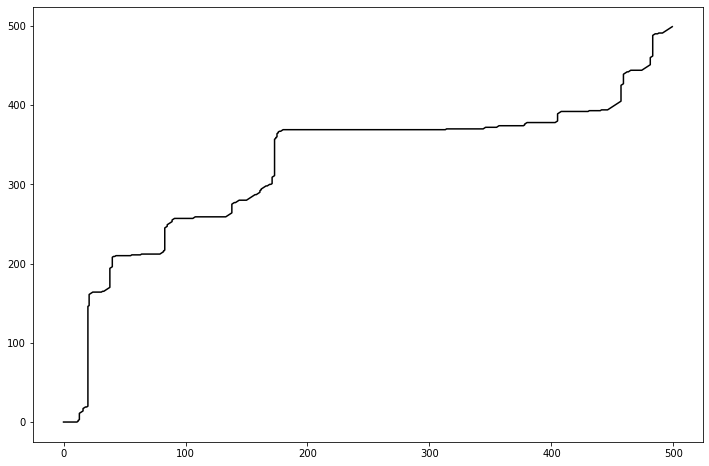
\includegraphics[width=10cm]{figuras/x0319_warp_path_zoom.png}
\caption{Caminho da DTW para o espectro estelar e telúrico de X0319 no intervalo de 834nm a 841nm}
\label{fig:x0319-warp-path-zoom}
\end{figure}

\begin{figure}[H]
  \centering
  \subfloat[Modelo telúrico do Molefit de X0319]{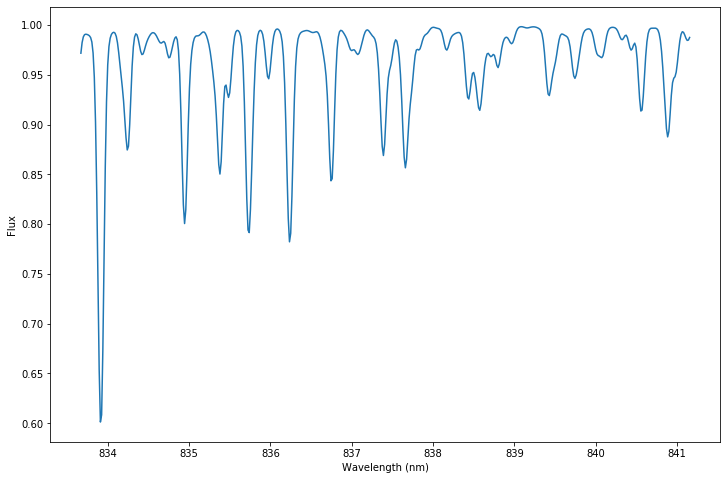
\includegraphics[width=0.5\textwidth]{figuras/x0319_v_o_e_tra_zoom.png}}
  \hfill
  \subfloat[Espectro telúrico de X0319 realinhado]{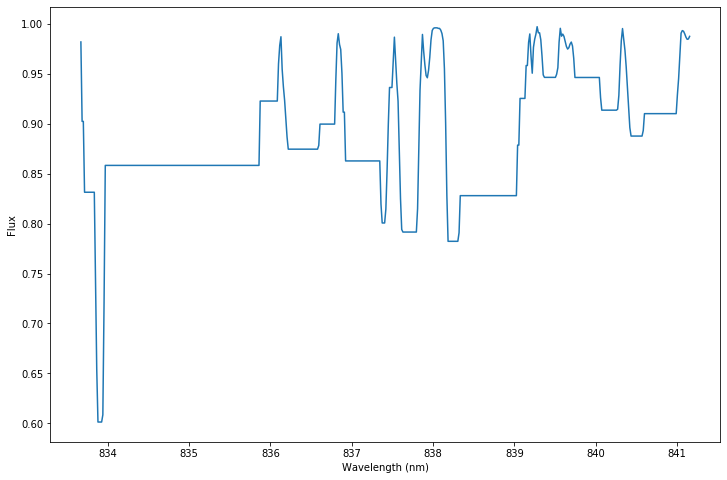
\includegraphics[width=0.5\textwidth]{figuras/x0319_v_o_e_aligned_zoom.png}}
  \caption{Espectro telúrico de X0319 e espectro telúrico realinhado a partir do caminho da DTW no intervalo de 834nm a 841nm}
  \label{fig:x0319-realigned-telluric-zoom}
\end{figure}

Neste experimento são observados os mesmos resultados dos experimentos anteriores em menor escala. Em um intervalo de comprimento de onda que abrange 9nm de espectro estelar ocorrem os mesmos deslocamentos horizontais e verticais no caminho da matriz de similaridades e no espectro telúrico realinhado também ocorre a formação de ângulos retos nas linhas de absorção.

% introduzir experimento seguinte

\section{DTW no sinal atmosférico}